\documentclass[12pt]{article}
\headsep 0.5 true cm
\topmargin 0pt
\oddsidemargin 0pt
\evensidemargin 0pt
\textheight 220mm
\textwidth 160mm
\renewcommand\baselinestretch{1.2}
\renewcommand\arraystretch{1.2}
\setlength{\parindent}{2em}
\usepackage{ctex}
\usepackage{CJK}
\usepackage{eucal}
\usepackage{amsfonts}
\usepackage{graphicx}
\usepackage{subfigure}
\usepackage{amssymb}
\usepackage{amsmath}
\begin{document}
%--------------------文章头------------------------
\vspace*{0.4cm}
\begin{center}
{
{\LARGE\heiti 三次样条插值}}\\[0.6cm]
{\normalsize 段晨光,\quad 龙华君}\\[0.1cm]
\end{center}
%--------------------摘要--------------------------
{\small
\noindent {\heiti 摘 \quad 要:}%
\parbox[t]{13.3cm}{ 
本文介绍了三次样条插值的定解条件与理论推导,给出了基于追赶法和修正追赶法的三次样条插值算法.进一步分析了三次样条插值的收敛性与稳定性,并针对等距节点高次多项式插值所出现的Runge现象和数值不稳定问题给出解决方案. 最后,给出数值算例,验证三次样条插值的收敛性与数值稳定性,并与等距节点高次多项式插值、Chebyshev插值对比,说明所给解决方案的有效性. }\\}	

{\small }	

{\small
\noindent
{\heiti 关键词:} { 三次样条插值} { 追赶法} { Runge现象} { Lebesgue常数} { Lagrange插值} { Chebyshev插值}}	
%-------------------正文------------------------------
\section*{{\large\bf 1}\quad\large\heiti  引言}	
\par 利用简单函数近似复杂函数,甚至解析形式未知的函数是计算数学中的基础问题,在数据建模、函数求值、数值微分、数值积分和微分方程数值解等问题中发挥重要作用. 花费尽可能少的时间和空间成本,尽可能精确稳定地近似目标函数是算法设计的目标.
\par 多项式插值形式简单,算法效率高,但是等距节点高次多项式插值会带来不可忽视的误差. 一方面,对于不满足复解析的函数,等距节点高次多项式插值会产生Runge现象,随着节点数增多,插值函数在插值区间边缘附近不收敛到目标函数,产生剧烈振荡. 此外,即便对于性质足够好的函数,随着节点数增多,等距高次多项式插值依旧会出现数值不稳定现象.这种不稳定现象由Lebesgue常数刻画,理论证明,等距节点的Lebesgue常数随着节点个数的增多而指数级变大. 
\par 针对等距节点高次多项式插值中出现的问题,主要有两种解决思路:改变插值节点位置,在奇异振荡出现的区间边缘附近节点加密,如Chebyshev插值、Sinc节点插值[1]等.用分段低次多项式代替高次多项式插值,如分段Lagrange插值,分段Hermit插值,分段样条插值等. 对于前者,理论证明,Lebesgue常数随插值节点的增多而增长的速度至少为对数级. 所以,节点的选择尽管可以大大提升数值稳定性,但是当节点规模变大,误差的传播依旧是不可忽视的. 更重要的是,对于不光滑甚至不连续的函数,整体插值依旧存在问题. 而且,实际计算中要求测量数据点满足特定分布分布往往是苛刻的. 对于后者,分段Lagrange插值彻底阻断了误差的传播,但是难以满足插值函数的导数连续性;分段Hermit插值同样无法保证二阶导数连续性,并且需要已知节点处的导数信息. 考虑到数值微分的不适定性,不论是实际测量还是预先计算,导数信息引入的较大误差都是无法避免的. 三次样条插值虽然无法彻底截断误差,但是可以保证误差的局部传播性,也保证了插值函数的二阶连续可微.
\par 本文主要围绕三次样条插值. 给出了三次样条插值的定解条件,并给出不同条件下的理论推导,分析问题的适定性. 进一步,给出求解算法并分析算法复杂性. 最后,不加严格证明地给出三次样条的收敛性与稳定性的分析,设计数值算例进行验证,与等距节点Lagrange插值、Chebyshev插值进行比较. 
\par 本文内容按如下方式组织:第二部分给出三次样条插值的问题描述与定解条件,在第三部分中给出对应的理论推导,分析了问题的适定性. 第四部分介绍具体算法,并分析算法复杂性. 第五部分略去严格理论证明,直观解释三次样条函数的收敛性与稳定性,并在通过数值实验验证. 第六部分为本文结论.

\section*{{\large\bf 2}\quad\large\heiti  问题定义}
\par 考虑到高次多项式带来的误差,我们采用分段插值的思想,使得误差不会被明显传播放大. 同时,我们希望得到的插值函数尽可能光滑,所需要的信息,特别是导数信息尽可能少.

\textbf{三次样条插值} 
给定$n+1$个插值点$\{(x_{i},y_{i})\}_{i=0}^n$,其中$a=x_{0}<x_{1}<...<x_{n}=b$,
满足$S(x_{i})=y_{i}$,
且$S(x)\in C^{2}$,
$S(x)\big|_{[x_{i-1},x_{i}]}\in\mathbb{P}_{3}$.

\par 不难发现,上述条件不足以唯一确定一分段多项式的所有参数. 实际应用中,下列条件往往作为定解条件.

\textbf{(1)简支边界条件}
	\begin{equation}\label{1}
	S'(a)=m_{0}, S'(b)=m_{n}
	\end{equation}
	
\textbf{(2)固支边界条件}
	\begin{equation}\label{2}
	S''(a)=M_{0}, S''(b)=M_{n}
	\end{equation}
	特别的,若$M_{0}=M_{1}=0$则称为自然边界条件.
	
\textbf{(3)周期边界条件}
	\begin{equation}\label{3}
	S'(a)=S'(b), S''(a)=S''(b)
	\end{equation}

\section*{{\large\bf 3}\quad\large\heiti  理论推导}
\subsection*{{\normalsize 3.1}\quad\normalsize\heiti 简支边界条件}
记$S^{''}(x)$在$x_{i}$点的值为$M_{i}(i=0,1,2,\cdots,n)$,$h_{i}=x_{i}-x_{i-1}(i=1,2,\cdots,n)$,当给定的定解条件为$S^{''}_{a}=M_0,S^{''}_{b}=M_n$时:
\par 在$x\in{[x_{i-1},x_{i}]}$上,由已知条件$S(x_{i-1})=y_{i-1}$以及$S^{''}(x_{i-1})=M_{i-1}$可得:
$$S(x)=y_{i-1}+\alpha(x-x_{i-1})+\cfrac{M_{i}}{2}(x-x_{i-1})^{2}+\beta(x-x_{i-1})^{3},$$
再由$S(x_{i})=y_{i},S^{''}(x_{i})=M_{i}$可得:
$$\alpha=\cfrac{y_{i}-y_{i-1}}{h_{i}}-\cfrac{M_{i}+2M_{i-1}}{6}h_{i},\beta=\cfrac{M_{i}-M_{i-1}}{6h_{i}}.$$
在区间$[x_{i-1},x_{i}]$内,有:
$$S^{'}(x_{i})=\cfrac{y_{i}-y_{i-1}}{h_{i}}+\cfrac{2M_{i}+M_{i-1}}{6}h_{i},$$
在区间$[x_{i},x_{i+1}]$内,有:
$$S^{'}(x_{i})=\cfrac{y_{i+1}-y_{i}}{h_{i+1}}-\cfrac{M_{i+1}+2M_{i}}{6}h_{i+1}.$$
由$S(x)$的一阶连续性$S^{'}(x_{i}-0)=S^{'}(x_{i}+0)$:
$$
\cfrac{y_{i}-y_{i-1}}{h_{i}}+\cfrac{2M_{i}+M_{i-1}}{6}h_{i}=\cfrac{y_{i+1}-y_{i}}{h_{i+1}}-\cfrac{M_{i+1}+2M_{i}}{6}h_{i+1},
$$
化简可得:
\begin{equation}\label{4}
h_{i}M_{i-1}+2(h_{i}+h_{i+1})M_{i}+h_{i+1}M_{i+1}=\cfrac{6(y_{i+1}-y_{i})}{h_{i+1}}-\cfrac{6(y_{i}-y_{i-1})}{h_{i}}.
\end{equation}
其中,$i=1,2,\cdots,n-1$,可得$n-1$个方程,写成如下矩阵形式为:
$$
\left[ \begin{matrix}
2(h_{2}+h_{1}) & h_{2} & 0 & \cdots & 0 & 0\\
h_{2} & 2(h_{3}+h_{2}) & h_{3} & \cdots & 0 & 0\\
\vdots & \vdots & \vdots & \ddots &\vdots &\vdots\\
0 & 0 & 0 &\cdots & h_{n-1} & 2(h_{n}+h_{n-1})\\
\end{matrix} \right]
\left[ \begin{matrix}
M_{1} \\
M_{2} \\
\vdots \\
M_{n-1} \\
\end{matrix} \right]
=$$
\begin{equation}\label{5}
\left[ \begin{matrix}
\cfrac{6(y_{2}-y_{1})}{h_{2}}-\cfrac{6(y_{1}-y_{0})}{h_{1}}-h_{1}M_{0}\\
\cfrac{6(y_{3}-y_{2})}{h_{3}}-\cfrac{6(y_{2}-y_{1})}{h_{2}}\\
\vdots\\
\cfrac{6(y_{n}-y_{n-1})}{h_{n}}-\cfrac{6(y_{n-1}-y_{n-2})}{h_{n-1}}-h_{n}M_{n}\\
\end{matrix} \right]
\end{equation}


\subsection*{{\normalsize 3.2}\quad\normalsize\heiti 固支边界条件}

记$S^{'}(x)$在$x_{i}$点的值为$m_{i}(i=0,1,2,\cdots,n)$,$h_{i}=x_{i}-x_{i-1}(i=1,2,\cdots,n)$,当给定的定解条件为$S^{'}_{a}=m_0$,$S^{'}_{b}=m_n$时:
\par 在$x\in{[x_{i-1},x_{i}]}$时,由已知条件$S(x_{i-1})=y_{i-1}$以及$S^{'}(x_{i-1})=m_{i-1}$可得:
$$S(x)=y_{i-1}+m_{i-1}(x-x_{i-1})+\alpha(x-x_{i-1})^{2}+\beta(x-x_{i-1})^{3},$$
再由$S(x_{i})=y_{i},S^{'}(x_{i})=m_{i}$可得:
$$\alpha=\cfrac{m_{i-1}+2m_{i}}{h_{i}}+\cfrac{3(y_{i}-y_{i-1})}{h_{i}^{2}},$$
$$\beta=\cfrac{m_{i-1}+m_{i}}{h_{i}^{2}}+\cfrac{2(y_{i-1}-y_{i})}{h_{i}^{3}}.$$
在区间$[x_{i-1},x_{i}]$内,有:
$$S^{''}(x_{i})=2\left[\cfrac{m_{i-1}+2m_{i}}{h_{i}}+\cfrac{3(y_{i}-y_{i-1})}{h_{i}^{2}}\right]+6\left[\cfrac{m_{i-1}+m_{i}}{h_{i}}+\cfrac{2(y_{i-1}-y_{i})}{h_{i}^{2}}\right ],$$
在区间$[x_{i},x_{i+1}]$内,有:
$$S^{''}(x_{i})=2\left [\cfrac{m_{i}+2m_{i+1}}{h_{i+1}}+\cfrac{3(y_{i+1}-y_{i})}{h_{i+1}^{2}}\right ].$$
由$S(x)$的二阶连续性可知$S^{''}(x_{i}-0)=S^{''}(x_{i}+0)$,有:
$$\cfrac{m_{i-1}+2m_{i}}{h_{i}}+\cfrac{3(y_{i}-y_{i-1})}{h_{i}^{2}}+3\left [\cfrac{m_{i-1}+m_{i}}{h_{i}}+\cfrac{2(y_{i-1}-y_{i})}{h_{i}^{2}}\right ]=\cfrac{m_{i}+2m_{i+1}}{h_{i+1}}+\cfrac{3(y_{i+1}-y_{i})}{h_{i+1}^{2}},
$$
化简可得:
\begin{equation}\label{6}
h_{i+1}m_{i-1}+2(h_{i}+h_{i+1})m_{i}+h_{i}m_{i+1}=\cfrac{3h_{i}}{h_{i+1}}(y_{i+1}-y_{i})+\cfrac{3h_{i+1}}{h_{i}}(y_{i}-y_{i-1}).
\end{equation}
其中,$i=1,2,\cdots,n-1$,可得$n-1$个方程,写成如下矩阵形式为:
$$
\left[ \begin{matrix}
2(h_{2}+h_{1}) & h_{1} & 0 & \cdots & 0 & 0\\
h_{3} & 2(h_{3}+h_{2}) & h_{2} & \cdots & 0 & 0\\
\vdots & \vdots & \vdots & \ddots &\vdots &\vdots\\
0 & 0 & 0 &\cdots & h_{n} & 2(h_{n}+h_{n-1})\\
\end{matrix} \right]
\left[ \begin{matrix}
m_{1} \\
m_{2} \\
\vdots \\
m_{n-1} \\
\end{matrix} \right]
=$$
\begin{equation}\label{7}
\left[ \begin{matrix}
\cfrac{3h_{1}}{h_{2}}(y_{2}-y_{1})+\cfrac{3h_{2}}{h_{1}}(y_{1}-y_{0})-h_{1}m_{0}\\
\cfrac{3h_{2}}{h_{3}}(y_{3}-y_{2})+\cfrac{3h_{3}}{h_{2}}(y_{2}-y_{1})\\
\vdots\\
\cfrac{3h_{n-1}}{h_{n}}(y_{n}-y_{n-1})+\cfrac{3h_{n}}{h_{n-1}}(y_{n-1}-y_{n-2})-h_{n-1}m_{n}\\
\end{matrix} \right]
\end{equation}

\subsection*{{\normalsize 3.3}\quad\normalsize\heiti 周期边界条件}

记$S^{'}(x)$在$x_{i}$点的值为$m_{i}$,$S^{''}(x)$在$x_{i}$点的值为$M_{i}(i=0,1,2,\cdots,n)$,$h_{i}=x_{i}-x_{i-1}(i=1,2,\cdots,n)$,当给定的定解条件为$S^{''}(a)=S^{''}(b)$,$S^{'}(a)=S^{'}(b)$时:
\par 在$x\in[x_{i-1},x_{i}]$时,可由简支边界相同的情况得到:
$$S(x)=y_{i-1}+\alpha(x-x_{i-1})+\cfrac{M_{i}}{2}(x-x_{i-1})^{2}+\beta(x-x_{i-1})^{3},$$
$$
\alpha=\cfrac{y_{i}-y_{i-1}}{h_{i}}-\cfrac{M_{i}+2M_{i-1}}{6}h_{i}, \beta=\cfrac{M_{i}-M_{i-1}}{6h_{i}}.
$$
在区间$[x_{i-1},x_{i}]$内,有:
$$S^{'}(x_{i})=\cfrac{y_{i}-y_{i-1}}{h_{i}}+\cfrac{2M_{i}+M_{i-1}}{6}h_{i},$$
可得:
$$m_{0}=\cfrac{y_{1}-y_{0}}{h_{1}}+\cfrac{2M_{1}+M_{0}}{6}h_{1},$$
$$m_{n}=\cfrac{y_{n}-y_{n-1}}{h_{n}}+\cfrac{2M_{n}+M_{n-1}}{6}h_{n}.$$
由已知条件$S^{'}(a)=S^{'}(b),S^{''}(a)=S^{''}(b)$可得:
$$\cfrac{y_{1}-y_{0}}{h_{1}}+\cfrac{2M_{1}+M_{n}}{6}h_{1}=\cfrac{y_{n}-y_{n-1}}{h_{n}}+\cfrac{2M_{n}+M_{n-1}}{6}h_{n},$$
化简得:
\begin{equation}\label{8}
-2h_{1}M_{1}+(2h_{n}-h_{1})M_{n}+h_{n}M_{n-1}=6\cfrac{y_{1}-y_{0}}{h_{1}}-6\cfrac{y_{n}-y_{n-1}}{h_{n}}.
\end{equation}
由$S(x)$的一阶导的连续性亦可得:
\begin{equation}\label{9}
\cfrac{y_{i}-y_{i-1}}{h_{i}}+\cfrac{2M_{i}+M_{i-1}}{6}h_{i}=\cfrac{y_{i+1}-y_{i}}{h_{i+1}}-\cfrac{M_{i+1}+2M_{i}}{6}h_{i+1}.
\end{equation}
其中,$i=1,2,\cdots,n-1$,总可得n个方程,写成如下矩阵形式为:
$$
\left[ \begin{matrix}
2(h_{2}+h_{1}) & h_{2} & 0 & \cdots & 0 & h_{1}\\
h_{2} & 2(h_{3}+h_{2}) & h_{3} & \cdots & 0 & 0\\
\vdots & \vdots & \vdots & \ddots &\vdots &\vdots\\
0 & 0 & 0 &\cdots & 2(h_{n}+h_{n-1}) & h_{n}\\
-2h_{1} & 0 & 0 & \cdots & h_{n} & 2h_{n}-h_{1}\\
\end{matrix} \right]
\left[ \begin{matrix}
M_{1} \\
M_{2} \\
\vdots \\
M_{n-1} \\
M_{n} \\
\end{matrix} \right]
=$$
\begin{equation}\label{10}
\left[ \begin{matrix}
\cfrac{6(y_{2}-y_{1})}{h_{2}}-\cfrac{6(y_{1}-y_{0})}{h_{1}}\\
\cfrac{6(y_{3}-y_{2})}{h_{3}}-\cfrac{6(y_{2}-y_{1})}{h_{2}}\\
\vdots\\
\cfrac{6(y_{n}-y_{n-1})}{h_{n}}-\cfrac{6(y_{n-1}-y_{n-2})}{h_{n-1}}\\
6\cfrac{y_{1}-y_{0}}{h_{1}}-6\cfrac{y_{n}-y_{n-1}}{h_{n}}\\
\end{matrix} \right]
\end{equation}


\subsection*{{\normalsize 3.4}\quad\normalsize\heiti 问题适定性分析}
\par 可以发现,对三种边界问题的求解,最后都归结于求解三对角线性方程组的问题. 下面将通过讨论线性代数方程组的性态得到三次样条插值的性态.
\par 由条件(1)(2)(3)下的三次样条插值与方程(5)(7)(10)的等价性可得以下结论:
\par \textbf{命题} 
在(1)(2)(3)任一条件下的三次样条插值都存在唯一.
\par 下讨论问题的病态性性. 不失一般性,讨论等距节点非周期样条插值对应的三对角阵条件数.
\par \textbf{命题} 
非周期边界条件等距节点三次样条插值的系数矩阵条件数不大于$\sqrt{3}$.
\par 以下简要介绍该条件数的估计:
当给定的是等距节点时,有$h_{i}=h(i=1,2,\cdots,n)$,则对应的系数矩阵为常数倍的:
$$
\left(\begin{matrix}
4 & 1 & 0 & \cdots & 0\\
1 & 4 & 1 & \cdots & 0\\
\vdots & \vdots & \ddots & \ddots & \vdots\\
0 & 0 & 0 & \cdots & 4\\
\end{matrix}\right)
$$	
可求出其对应的特征值与特征向量为:
$$\lambda_{j}=4h+2h\cos \cfrac{j\pi}{n},$$ 
$$x_{j}=\left(\sin\cfrac{j\pi}{n},\sin\cfrac{2j\pi}{n},\cdots,\sin\cfrac{(n-1)j\pi}{n}\right)^{T}, $$
其中,$j = 1,2,\cdots,n-1$.
所以$$\lambda_{max}\leq6h,\lambda_{min}\geq2h,$$
故矩阵条件数
$$cond=\cfrac{\lambda_{max}}{\lambda_{min}}\leq\sqrt{3}.$$
\par 上述命题说明,三次样条插值是存在唯一,并且良态的.

\section*{{\large\bf 4}\quad\large\heiti  算法设计}
\par 考虑到理论推导得到的线性代数方程组的带状特性,主要思路为采用追赶法求解.
\subsection*{{\normalsize 4.1}\quad\normalsize\heiti 追赶法}
\par 对于求解简支边界条件与固支边界条件的问题,都形同与求解如下一个线性代数方程组:
$$
\left[ \begin{matrix}
 b_{1} & c_{1} & 0 & 0 & 0 & \cdots & \cdots& 0\\
 a_{2} & b_{2} & c_{2} & 0 & 0 & \cdots & \cdots & 0\\
 0 & a_{3} & b_{3} &c_{3} & 0 & \cdots & \cdots & 0\\
 \vdots & \vdots & \vdots & \vdots & \ddots & \ddots & \ddots & \vdots\\  
 0 & 0 & 0 & 0 & \cdots & \cdots & a_{n} & b_{n}\\
 \end{matrix} \right]
 \left[ \begin{matrix} 
 x_{1}\\
 x_{2}\\
 x_{3}\\
 \vdots\\
 x_{n}\\
 \end{matrix} \right]
 =
 \left[ \begin{matrix}
 d_{1}\\
 d_{2}\\
 d_{3}\\
 \vdots\\
 d_{n}\\
 \end{matrix} \right]
$$	
其计算程序为先形成$\{q_{k}\}$和$\{u_{k}\}$:
\begin{equation}\label{11}
\begin{cases}
	p_{k}=a_{k}q_{k-1}+b_{k} & q_{0} = 0\\
	q_{k}=-\cfrac{c_{k}}{p_{k}} &\\
	u_{k}=\frac{1}{p_{k}}(d_{k}-a_{k}u_{k-1}) & u_{0}=0\\
\end{cases}
\end{equation}
然后按下述关系式逐一推导各$x_{j}$的值:
\begin{equation}\label{12}
\begin{cases}
	x_{k}=q_{k}x_{k+1}+u_{k} & k=1,2,\cdots,n-1\\
	x_{n}=u_{n}\\
\end{cases}
\end{equation}

\subsection*{{\normalsize 4.2}\quad\normalsize\heiti 修正追赶法} 
对于求解周期边界条件问题形如求解如下线性方程组,其一般形式为:
$$
\left[ \begin{matrix}
b_{1} & c_{1} & 0 & 0 & 0 & \cdots & \cdots& a_{1}\\
a_{2} & b_{2} & c_{2} & 0 & 0 & \cdots & \cdots & 0\\
0 & a_{3} & b_{3} &c_{3} & 0 & \cdots & \cdots & 0\\
\vdots & \vdots & \vdots & \vdots & \ddots & \ddots & \ddots & \vdots\\
0 & 0 & 0 & 0 & \cdots & \cdots & b_{n-1} & c_{n-1}\\ 
c_{n} & 0 & 0 & 0 & \cdots & \cdots & a_{n} & b_{n}\\
\end{matrix} \right]
\left[ \begin{matrix} 
x_{1}\\
x_{2}\\
x_{3}\\
\vdots\\
x_{n-1}\\
x_{n}\\
\end{matrix} \right]
=
\left[ \begin{matrix}
d_{1}\\
d_{2}\\
d_{3}\\
\vdots\\
d_{n-1}\\
d_{n}\\
\end{matrix} \right]	
$$
其计算程序[2]为先按(11)计算出$\{p_{k}\},\{q_{k}\},\{u_{k}\}$. 再按下述公式算出$t_{k}和u_{k}$:
\begin{equation}\label{13}
\begin{cases}
	s_{k}=-\cfrac{1}{p_{k}}(a_{k}s_{k-1}), & s_{0}=1,\\
	t_{k}=q_{k}t_{k+1}+s_{k}, & t_{n}=1,\\
	v_{k}=q_{k}v_{k+1}+u_{k}, & v_{n}=0.\\
\end{cases}
\end{equation}
接着从方程:
\begin{equation}\label{14}
c_{n}(t_{1}x_{n}+v_{1})+a_{n}(t_{n-1}x_{n}+v{n-1})+b_{n}x_{n}=d_{n},
\end{equation}
解出$x_{n}$,最后用递推关系式:
\begin{equation}\label{15}
x_{k}=t_{k}x_{n}+v_{n}, 
\end{equation}
其中$(k=1,\cdots,n-1)$,逐个求出$x_{n-1},\cdots,x_{1}$.

\subsection*{{\normalsize 4.3}\quad\normalsize\heiti 算法分析} 
\par 算法复杂度分析
追赶法求解三对角方程组的运算复杂度为$O(n)$,并且在储存方面,只需存储一个4个$n$维的向量,大大减少了直接存储一个矩阵所带来的存储浪费.

\section*{{\large\bf 5}\quad\large\heiti  若干性质与数值验证}
\par 不失一般性,文中所有数值实验均基于简支边界条件,问题对边界条件的稳定性(5.3.2中验证)保证了这样做的合理性.
\par 
\subsection*{{\normalsize 5.1}\quad\normalsize\heiti Runge现象} 
\subsubsection*{{\small 5.1.1}\quad\small\heiti 理论分析}
\par 直观地,Runge现象由于[3]函数高阶导数的数量级随着阶数的增大快速增大,导致误差函数在边缘附近不收敛到$0$. 事实上,对函数$f(x)$的等距节点Language插值的余项估计:
$$\mathop{\max}_{-1\leq x \leq 1} | R(x) | \leq M_{n}\frac{h^{n}}{4n},$$
其中,
$$\mathop{\max}_{-1\leq x \leq 1} |f^{(n)}(x)|\leq M_{n}$$.
\par 对于Runge现象,主要有以下解决方法:
\par (1)改变插值节点:高次等距节点多项式插值引起的奇异振荡可以通过改变插值节点分布,使节点在区间边界处分布更加密集达到最小化.
\par 如,使用chebyshev节点代替等距节点,若函数$f(x)$及导函数$f'(x)$在区间$[-1,1]$连续,则$f(x)$的Chebyshev插值函数一致地收敛到$f(x)$.
\par  (2)使用分段多项式:避免Runge现象可以通过使用分段低次多项式,不出现误差估计中的高阶导数,问题不会随着插值节点个数的增大逐渐趋于病态.
\par 如,对于三次样条插值:类似Hermite插值的误差估计,在区间$[-1,1]$上,插值误差为
$$R(x)=\cfrac{f^{2n+2}(\eta)}{(2n+2)!}\prod_{i=0}^{n}(x-x_{i})^{2},$$
其中$\eta\in(-1,1).$所以,
$$||R(x)||_{\infty}\leq\cfrac{||f^{2n+2}(x)||_{\infty}}{(2n+2)!}\mathop{\max}_{-1\leq x \leq 1}\prod_{i=0}^{n}(x-x_{i})^{2}.$$
又
$$\mathop{\max}_{-1\leq x \leq 1}\prod_{i=0}^{n}(x-x_{i})^{2}\leq M_{1}(2n)!h^{2n},$$
$$||f^{2n+2}(x)||_{\infty}\leq M_{n},$$
所以
$$||R(x)||_{\infty}\leq C_{n}h^{2n+2}.$$
\par 特别的,当$n=1$时,对应三次样条插值,对任意$x\in[-1,1]$,有
$$||R(x)||_{\infty}\leq Ch^{4}.$$
保证了三次样条插值在整个区间上4阶收敛,避免Runge现象.
\par (3)约束最小化方法[3].
\subsubsection*{{\small 5.1.2}\quad\small\heiti 数值验证} 
\par 对函数$f(x)=\cfrac{1}{12x^{2}+1}$在区间$[-1,1]$等距节点插值,分别选取5,15,25个插值节点.

\begin{figure}[h]
	\subfigure[原函数]{\label{fig:subfig1:a}
		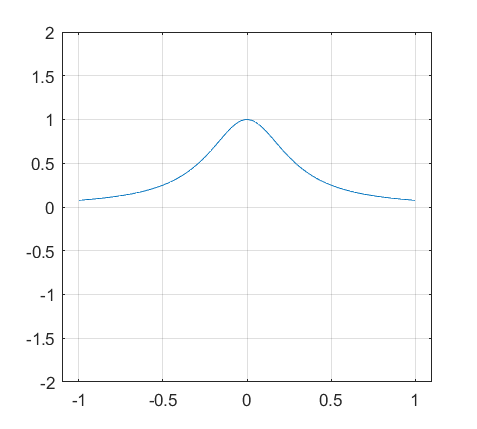
\includegraphics[width=0.22\textwidth]{figure//fig00.png}}
	\subfigure[5个等距节点]{\label{fig:subfig1:b}
		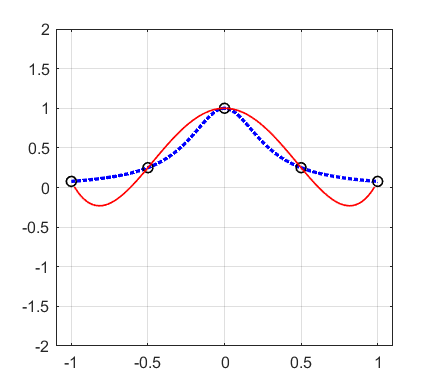
\includegraphics[width=0.22\textwidth]{figure//fig01.png}}
	\subfigure[15个等距节点]{\label{fig:subfig1:c}
		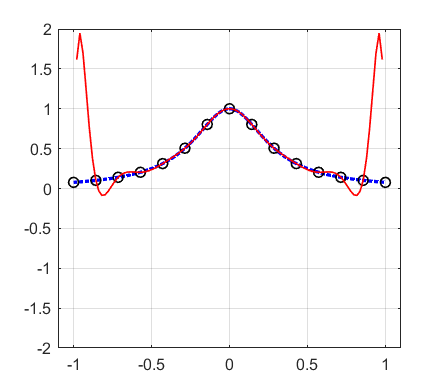
\includegraphics[width=0.22\textwidth]{figure//fig02.png}}
	\subfigure[25个等距节点]{\label{fig:subfig1:d}
		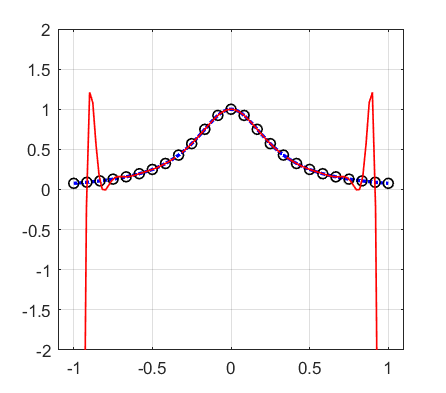
\includegraphics[width=0.22\textwidth]{figure//fig03.png}}
	\label{fig0003} 
	\caption{等距节点Lagrange插值}
\end{figure}

\par 从图1中可以发现,随着节点数的增多,区间中段的插值函数逐渐逼近原函数,但是在靠近区间边缘的位置,插值函数出现明显振荡,并且随着阶数的阶数逐渐变大.
\par 对函数$f(x)=\cfrac{1}{12x^{2}+1}$在区间$[-1,1]$选取25个节点,分别进行chebyshev插值,与三次样条插值.

\begin{figure}[h]
	\subfigure[chebyshev插值]{\label{fig:subfig2:a}
		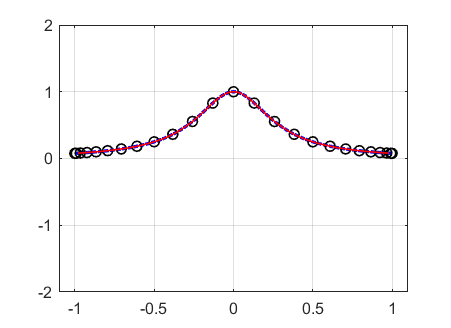
\includegraphics[width=0.5\textwidth]{figure//fig04.png}}
	\subfigure[等距节点三次样条插值]{\label{fig:subfig2:b}
		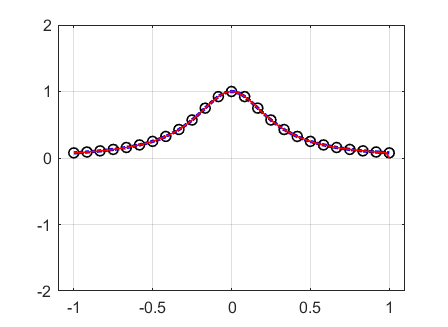
\includegraphics[width=0.5\textwidth]{figure//fig05.png}}
	\label{fig04} 
	\caption{消除Runge现象}
\end{figure}

\par 从图2中可以发现,Chebyshev节点在区间边缘附近分布密集,在区间中部分布稀疏. 不论Chebyshev插值还是等距节点三次样条插值,在整个区间上都很好地拟合曲线,没有出现Runge现象.
\par 事实上,由上述理论推导可得,三次样条插值具有4阶收敛,下面给出数值验证.
\par 若插值满足$\alpha$阶精度,即
$$||R(x)||_{\infty} \leq C h^{\alpha},$$
则有
$$log\left(||R(x)||_{\infty}\right) \leq logC + \alpha\cdot log h$$
故对得到的误差取对数关于节点间距的对数值进行线性最小二乘拟合,得到:
$$\hat{y} = 4.1660 \times x + 2.9478.$$

\begin{figure}[h]
	\subfigure[误差随节点间隔变化]{\label{fig:subfig2:a}
		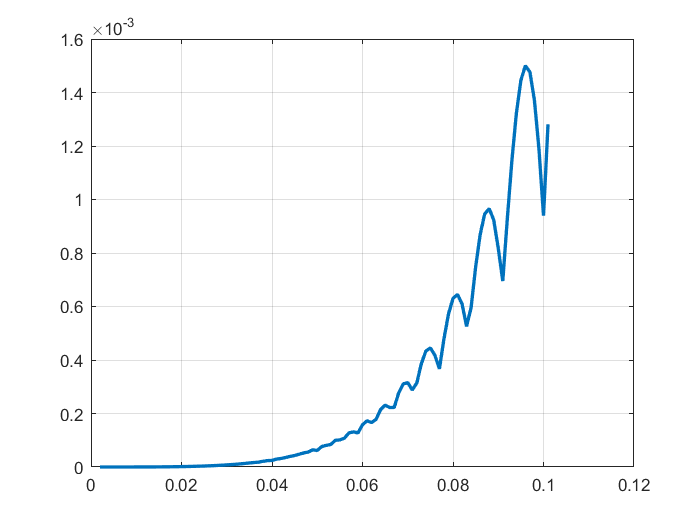
\includegraphics[width=0.5\textwidth]{figure//fig18.png}}
	\subfigure[误差对数随节点间隔对数的变化]{\label{fig:subfig2:b}
		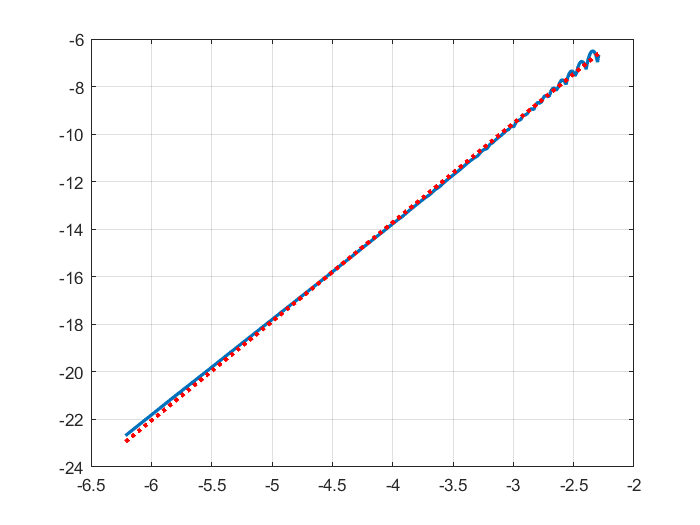
\includegraphics[width=0.5\textwidth]{figure//fig19.png}}
	\label{fig08} 
	\caption{插值函数随节点间距的收敛情况}
\end{figure}

从图3及计算得到的最小二乘估计可得,三次样条插值近似4阶收敛,与理论估计吻合.

\subsection*{{\normalsize 5.2}\quad\normalsize\heiti 等距高次插值的数值不稳定性}  
\subsubsection*{{\small 5.2.1}\quad\small\heiti 理论分析}
\par 多项式插值的数值稳定性由Lebesgue常数刻画,Lebesgue常数仅与节点类型与节点个数有关:
\par 等距节点的Lebesgue常数$\Lambda_{n}(E)$满足:
$$\Lambda_{n}(E)\geq \frac{2^{n-2}}{n^{}2},$$
\par chebyshev节点的Lebesgue常数$\Lambda_{n}(C)$满足:
$$\Lambda_{n}(C) \leq \frac{2}{\pi}ln(n+1)+1.$$
\par 用Chebyshev节点代替等距节点可以极大地降低Lebesgue常数,提高数值稳定性. 而三次样条插值由于其局部性质,使得误差不会被传播扩散,也具有很好的稳定性.

\par 

\subsubsection*{{\small 5.2.2}\quad\small\heiti 数值验证} 
\par 对函数$f(x)=sinx$在区间$[-1,1]$上分别使用60个等距节点Language插值、Chebyshev插值和等距节点三次样条插值.

\begin{figure}[h]
	\subfigure[原函数]{\label{fig:subfig3:a}
		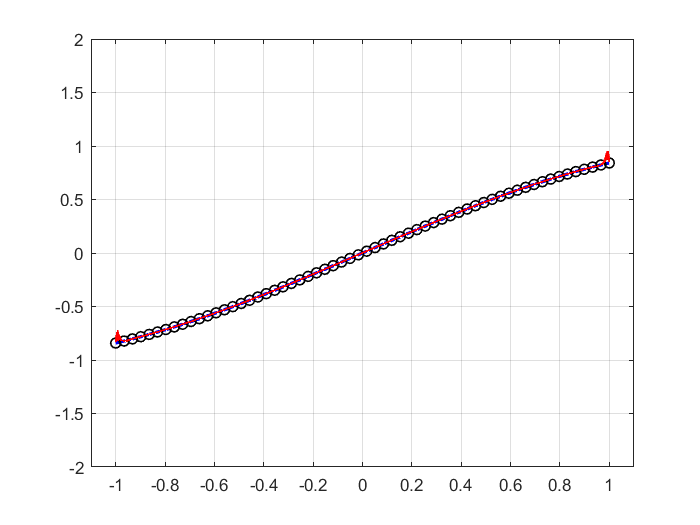
\includegraphics[width=0.22\textwidth]{figure//fig06.png}}
	\subfigure[等距节点插值(局部)]{\label{fig:subfig3:b}
		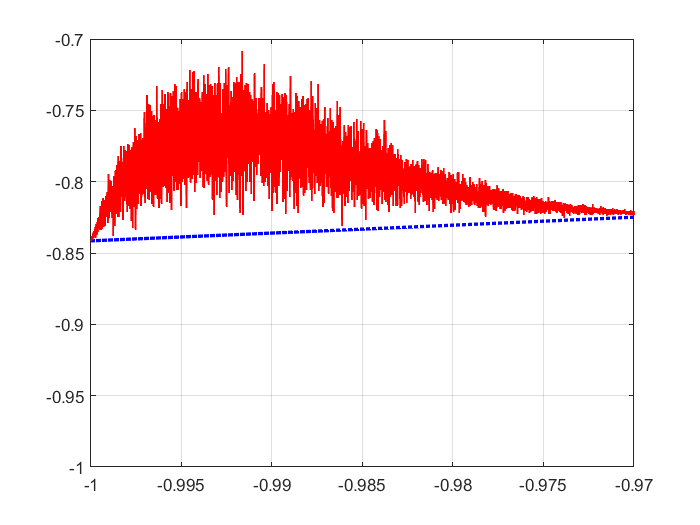
\includegraphics[width=0.22\textwidth]{figure//fig07.png}}
	\subfigure[chebyshev插值(局部)]{\label{fig:subfig3:c}
		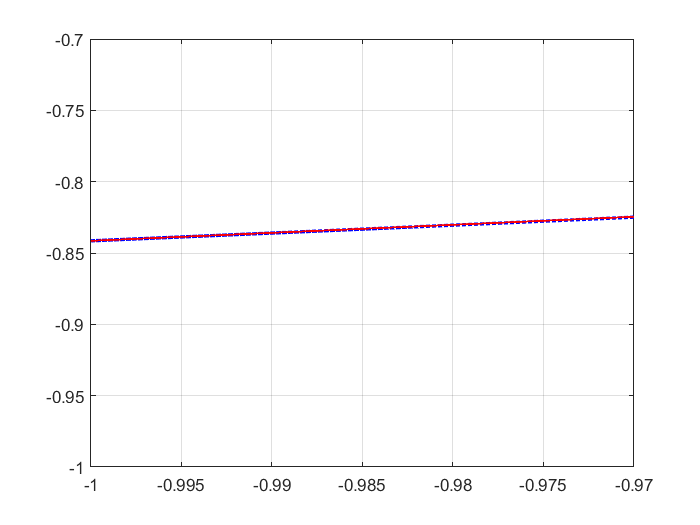
\includegraphics[width=0.22\textwidth]{figure//fig08.png}}
	\subfigure[三次样条插值(局部)]{\label{fig:subfig3:d}
		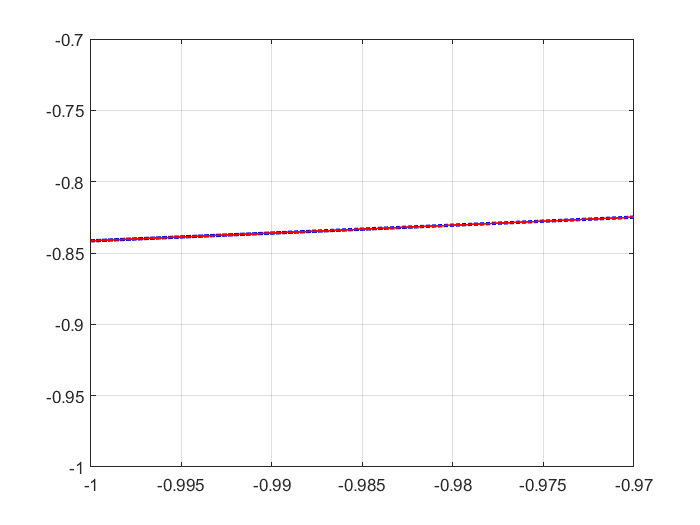
\includegraphics[width=0.22\textwidth]{figure//fig09.png}}
	\label{fig05} 
	\caption{不同插值方法对舍入误差的稳定性}
\end{figure}

\par 从图4(a)可得,当选取60个节点时,等距高次多项式插值在区间边缘附近出现明显误差. 图4(b)(c)(d)分别是等距节点、Chebyshev节点插值函数和三次样条插值函数在左端点附近的局部情形. 可见Chebyshev插值和三次样条插值可以有效提高插值的数值稳定性.

\subsection*{{\normalsize 5.3}\quad\normalsize\heiti 三次样条插值对条件的稳定性} 
\subsubsection*{{\small 5.3.1}\quad\small\heiti 理论分析} 
\par 实际计算中,数据本身的误差也是需要考虑的问题. 三次样条插值保证函数二阶连续可微,不是严格意义上的完全阻断误差传播. 另一方面,不管是实际测量还是利用数值微分估计边界条件,都会引入不可忽视的误差. 
\par 尽管如此,分段的性质保证三次样条插值不会使误差传播甚至放大.

\subsubsection*{{\small 5.1.2}\quad\small\heiti 数值验证} 
\par 对函数$f(x)=\cfrac{1}{12x^{2}+1}$在区间$[-1,1]$选取15个节点$\{(x_{i},y_{i})\}_{i=0}^{14}$,对$\{y_{i}\}_{i=0}^{14}$引入不同大小的$Gauss$噪声,
得到$\{(x_{i},\tilde{y_{i}})\}_{i=0}^{14}$,对扰动后的数据点三次样条插值.

\begin{figure}[h]
	\subfigure[$\epsilon=1.0 \times 10^{-4}$]{\label{fig:subfig4:a}
		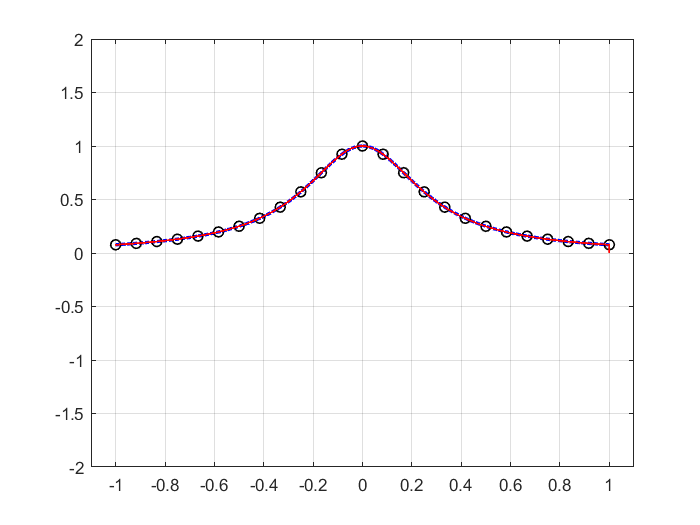
\includegraphics[width=0.22\textwidth]{figure//fig10.png}}
	\subfigure[$\epsilon=1.0 \times 10^{-3}$]{\label{fig:subfig4:b}
		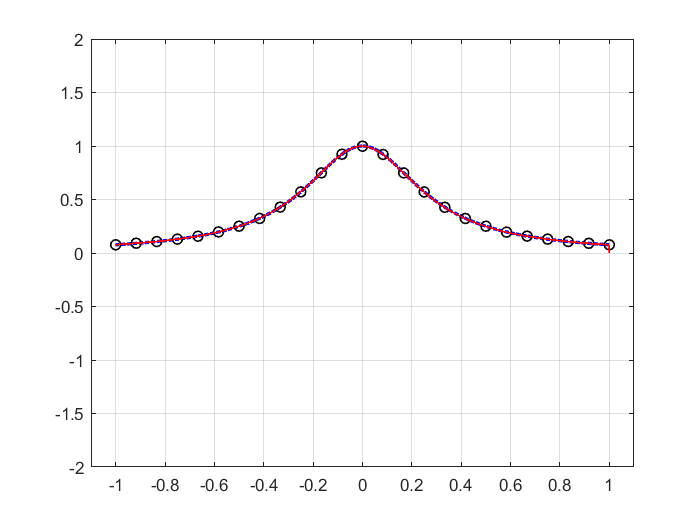
\includegraphics[width=0.22\textwidth]{figure//fig11.png}}
	\subfigure[$\epsilon=1.0 \times 10^{-2}$]{\label{fig:subfig4:c}
		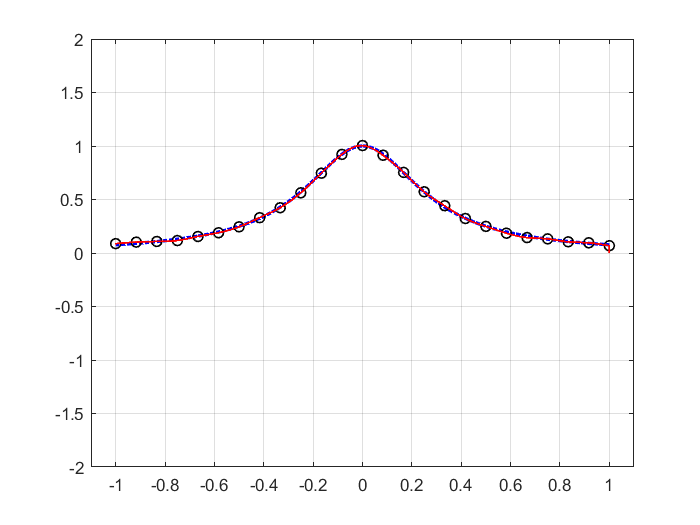
\includegraphics[width=0.22\textwidth]{figure//fig12.png}}
	\subfigure[$\epsilon=1.0 \times 10^{-1}$]{\label{fig:subfig4:d}
		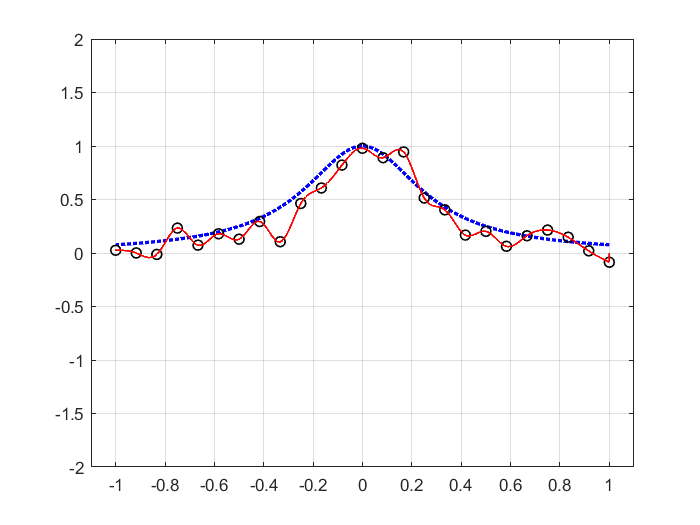
\includegraphics[width=0.22\textwidth]{figure//fig13.png}}
	\label{fig06} 
	\caption{在插值点引入不同大小随机扰动}
\end{figure}

\begin{table}[h]
\centering
\setlength{\abovecaptionskip}{10pt}
\caption{引入不同随机扰动带来误差$||R(x)||_{\infty}$}
\begin{tabular}{cccc}
\hline
$\epsilon=1.0 \times 10^{-4}$& $\epsilon=1.0 \times 10^{-3}$& 
$\epsilon=1.0 \times 10^{-2}$& $\epsilon=1.0 \times 10^{-1}$\\
\hline
$3.3226\times10^{-4}$& $1.2499\times10^{-3}$& 
$1.3256\times10^{-2}$& $1.9471\times10^{-1}$\\
\hline
\end{tabular}
\end{table}

\par 从图5和表1可以得到,三次样条插值函数对插值节点引入的随机扰动不敏感,具有很好的稳定性.

\par 对函数$f(x)=\cfrac{1}{12x^{2}+1}$在区间$[-1,1]$选取15个节点. 不失一般性,边界条件分别选择$M_{0}=M_{n}=100$、$M_{0}=M_{n}=50$、$M_{0}=M_{n}=10$、$M_{0}=M_{n}=0$.
所给条件进行三次样条插值.

\begin{figure}[h]
	\subfigure[{\tiny $M_{0}=100,M_{n}=100$}]{\label{fig:subfig5:a}
		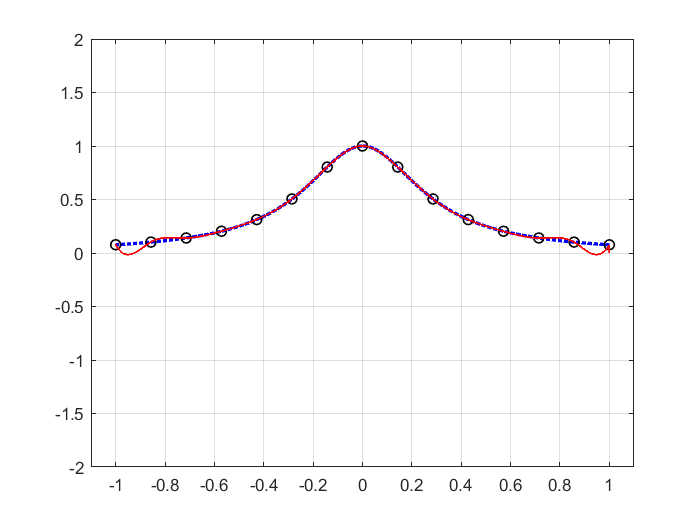
\includegraphics[width=0.22\textwidth]{figure//fig14.png}}
	\subfigure[{\tiny $M_{0}=50,M_{n}=50$}]{\label{fig:subfig5:b}
		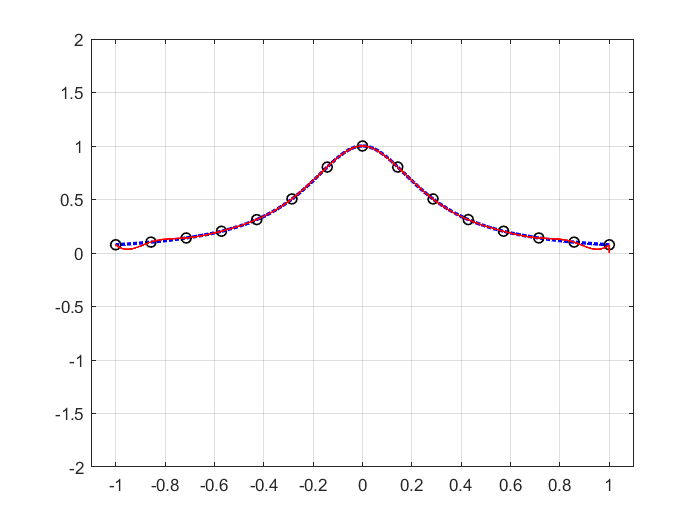
\includegraphics[width=0.22\textwidth]{figure//fig15.png}}
	\subfigure[{\tiny $M_{0}=10,M_{n}=10$}]{\label{fig:subfig5:c}
		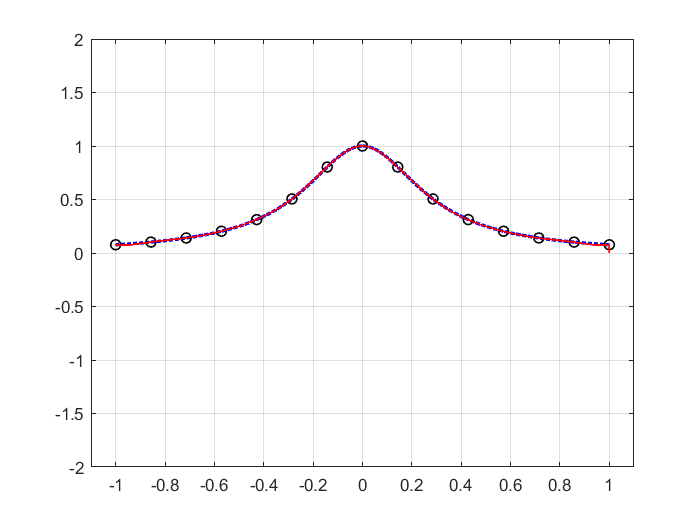
\includegraphics[width=0.22\textwidth]{figure//fig16.png}}
	\subfigure[{\tiny $M_{0}=0,M_{n}=0$}]{\label{fig:subfig5:d}
		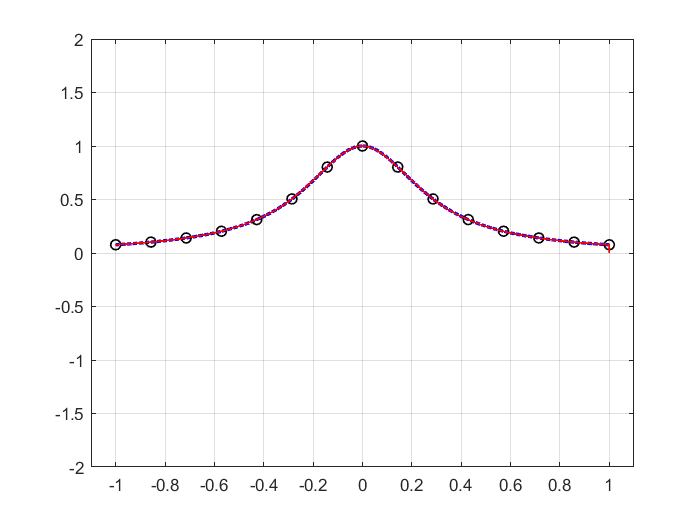
\includegraphics[width=0.22\textwidth]{figure//fig17.png}}
	\label{fig07} 
	\caption{不同边界条件的插值结果}
\end{figure}

\par 从图6看出,边界条件的选取直接地影响到始末两个子区间内的插值效果. 若分别删去开始两个连续子区间和末尾两个连续子区间,仅考虑剩余的拟合函数,最大模误差如表2.

\begin{table}[h]
	\centering
	\setlength{\abovecaptionskip}{10pt}
	\caption{不同边界条件下函数中段的误差$||R(x)||_{\infty}$}
	\begin{tabular}{cccc}
	\hline
	$M_{0}=100,M_{n}=100$& $M_{0}=50,M_{n}=50$& $M_{0}=10,M_{n}=10$& $M_{0}=10,M_{n}=10$\\
	\hline
	$3.2382\times10^{-3}$& $3.1770\times10^{-3}$& 
	$3.1281\times10^{-3}$& $3.1160\times10^{-3}$\\
	\hline
	\end{tabular}
\end{table}

\par 从表2可以得到,除相邻边界的区间之外,插值的精度并未受到边界值选取的影响. 可见,三次样条插值对边界条件不敏感.

\section*{{\large\bf 6}\quad\large\heiti  结论}
\par 本文主要讨论了三次样条插值. 我们给出了三次样条插值的三种不同定解条件,并给出相应条件下的理论推导,将插值问题转化为求解三对角方程或近似三对角方程的问题. 进一步,基于追赶法以及修正的追赶法,给出三次样条插值的求解算法并分析了算法复杂性. 此外,针对等距节点高次多项式插值中出现的Runge现象和Lebesgue常数过大引起的数值不稳定问题,我们给出了三次样条插值的解决方案,分析了方案的有效性并在数值算例中与等距节点Lagrange插值、Chebyshev插值对比插值效果,实验证明三次样条插值可以有效避免Runge现象并有很好的数值稳定性,并且验证了三次样条插值的4次收敛性. 最后,我们在插值节点加入多组不同大小的随机扰动,进一步验证了三次样条插值对插值条件误差的稳定性;分别给边界条件赋不同的值,说明了插值函数对边界条件误差的稳定性.
	
%-----------------------参考文献-----------------------	
{\footnotesize
\begin{thebibliography}{99}
\setlength{\itemsep}{0pt}
\setlength{\parskip}{0pt}
\bibitem{1}
Youssef M, El-Sharkawy HA, Baumann G. "Lebesgue Constant Using Sinc Points". \textit{Advances in Numerical Analysis}. September 2016:1-10. doi:10.1155/2016/6758283.
\bibitem{2}
王仁宏. 数值逼近[M]. 第2版.  北京 : 高等教育出版社, 2012
\bibitem{3}
Runge's phenomenon(Wikipedia)
\par https://en.wikipedia.org/wiki/Runge\%27s\_phenomenon.

\end{thebibliography}}	

%-----------------------附录-----------------------		

	
\end{document}
